% 导言区：格式定义
\documentclass[12pt,a4paper]{article} 
\usepackage{geometry} 
\geometry{left=2.5cm, right=2.5cm, top=2.5cm, bottom=2.5cm}
\usepackage{graphicx} 
\usepackage{float} 
\usepackage{booktabs} 
\usepackage{amsmath} 
\usepackage{amssymb}
\renewcommand{\baselinestretch}{1.15} 

% 引入超链接宏包
\usepackage[colorlinks=true, linkcolor=blue, urlcolor=blue, citecolor=blue]{hyperref}

% 强制所有段落首行缩进
\usepackage{indentfirst}
\setlength{\parindent}{2em} 

% ====== 目录与标题格式优化 ======
\usepackage{titlesec}
\titleformat{\section}[block]{\large\bfseries\filcenter}{\thesection.}{0.5em}{}
\titleformat{\subsection}[block]{\normalsize\bfseries\filcenter}{\thesubsection}{0.5em}{}
\renewcommand{\refname}{\large\bfseries\filcenter References}

% 文章主标题、作者、邮箱、代码链接、日期
\title{\textbf{\Large Multivariate Time Series Forecasting of PM2.5 Concentration Using Long Short-Term Memory (LSTM) Networks}} 
\author{
    Li Chao \\ 
    \href{mailto:superlee0183@gmail.com}{superlee0183@gmail.com} \\
    \vspace{0.1cm} \\
    \normalsize \textbf{Code:} \url{https://github.com/superlc0183/PRML2026}
} 
\date{April 18, 2026} 

\begin{document}
\maketitle 

\begin{abstract}
Predicting air pollution remains a critical challenge due to the complex, non-linear interplay of meteorological variables over time. In this report, we investigate the application of Long Short-Term Memory (LSTM) architecture to forecast PM2.5 concentrations based on a multivariate dataset from Beijing. By reframing continuous sensor data into a supervised learning structure and incorporating features such as dew point, temperature, pressure, and wind dynamics, we construct a 3D tensor-based neural network. The LSTM model demonstrates exceptional capability in capturing temporal dependencies, achieving a Root Mean Square Error (RMSE) of 25.663 on the test set. Through empirical validation, we confirm that integrating multiple meteorological variables significantly enhances the temporal forecasting accuracy compared to univariate analysis.
\end{abstract}

\newpage
\renewcommand{\contentsname}{\large\bfseries\filcenter Contents}
\tableofcontents
\newpage

\section{Introduction}
Time series forecasting is a crucial domain within Pattern Recognition and Machine Learning (PRML). Unlike standard regression tasks where data points are assumed to be independent, time series data possesses strict sequential dependencies. Traditional Feed-Forward Neural Networks fail to capture this temporal context. 

The objective of this study is to leverage an LSTM architecture—a specialized Recurrent Neural Network (RNN) designed to avoid the vanishing gradient problem—to predict future air pollution levels. We utilize the Beijing PM2.5 dataset from Kaggle, which logs hourly meteorological conditions and pollution levels over five years. The mission is to utilize multivariate historical data (at time $t-1$) to accurately predict the PM2.5 concentration at the subsequent hour (at time $t$).

\section{Methodology and Data Engineering}

\subsection{Data Preprocessing and Normalization}
The raw dataset consists of 43,800 hourly records without missing values. A preliminary visualization of the PM2.5 distribution across the five years is presented in Figure \ref{fig:trend}.

\begin{figure}[H]
    \centering
    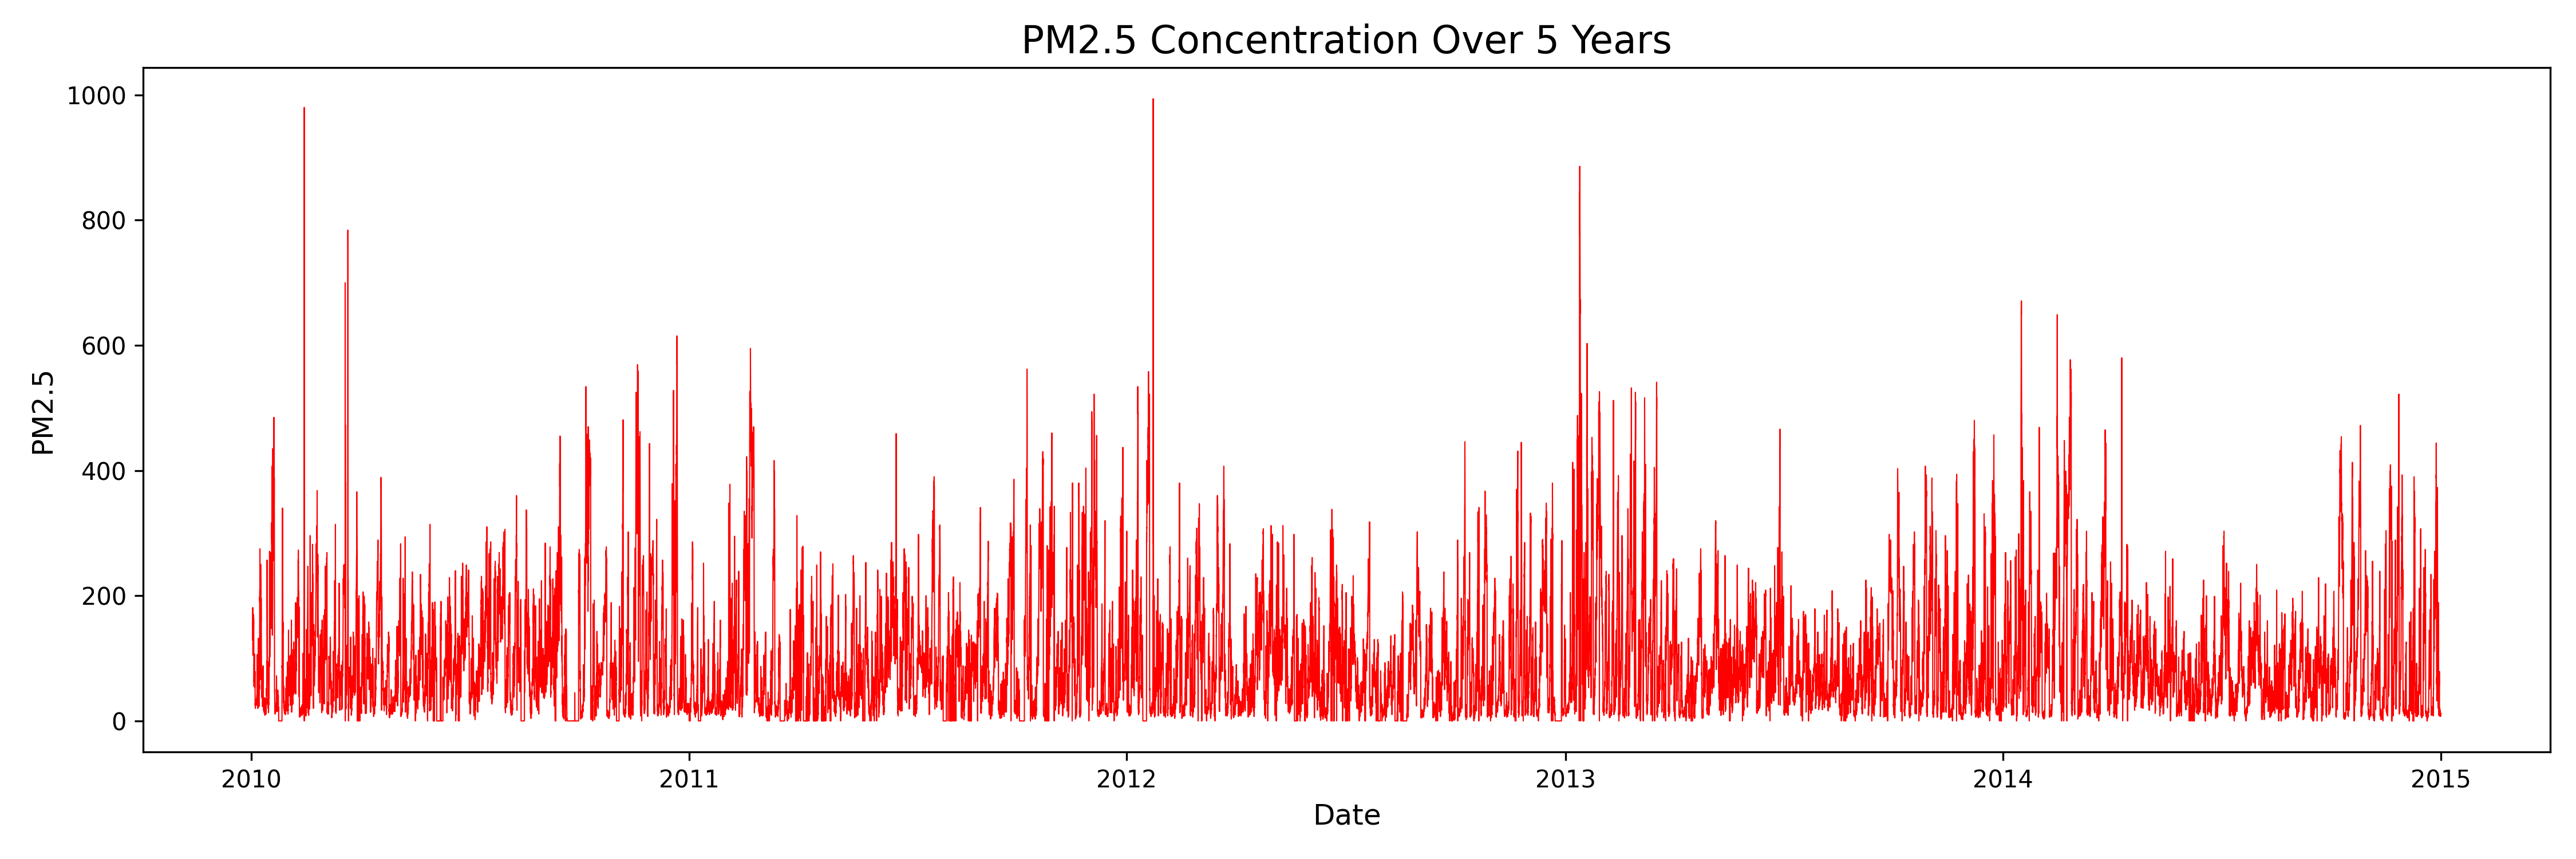
\includegraphics[width=\textwidth]{pm25_trend.png}
    \caption{\textbf{Overall Trend of PM2.5 Concentration Over 5 Years}}
    \label{fig:trend}
\end{figure}

To prepare the data for the neural network, two critical transformations were applied:
\begin{itemize}
    \item \textbf{Label Encoding:} Categorical variables, specifically the wind direction (\texttt{wnd\_dir}), were mapped to integer values utilizing \texttt{LabelEncoder}.
    \item \textbf{Min-Max Scaling:} Neural networks are highly sensitive to unscaled inputs, which can cause gradient explosions. All variables, including pressure (scale of $10^3$) and temperatures, were compressed into a $[0, 1]$ range via \texttt{MinMaxScaler}.
\end{itemize}

\subsection{Supervised Learning Framing}
LSTM networks strictly require a 3D input tensor with dimensions: \texttt{[samples, timesteps, features]}. We implemented a sliding window technique to restructure the time series into a supervised learning paradigm. The data at hour $t-1$ (8 features including past pollution and weather) acts as the input $X$, while the pollution concentration at hour $t$ serves as the target $Y$. The resulting training tensor shape was mapped to \texttt{[35040, 1, 8]}, representing the first four years of data.

\subsection{LSTM Network Architecture}
The model was constructed sequentially:
\begin{enumerate}
    \item \textbf{LSTM Layer:} Comprising 50 hidden units to capture the temporal representations.
    \item \textbf{Dense Layer:} A fully connected layer with a single output neuron to predict the continuous PM2.5 value.
    \item \textbf{Optimization:} The network was compiled using the Mean Absolute Error (MAE) loss function and optimized via the Adam optimizer algorithm for 50 epochs with a batch size of 72.
\end{enumerate}

\section{Experimental Results and Analysis}

\subsection{Training Dynamics}
Figure \ref{fig:loss} illustrates the training process. The model exhibited rapid convergence within the first three epochs. Most importantly, the validation loss tightly tracked the training loss throughout the 50 epochs, indicating a well-regularized network without symptoms of severe overfitting, successfully filtering out extreme meteorological stochasticity.

\begin{figure}[H]
    \centering
    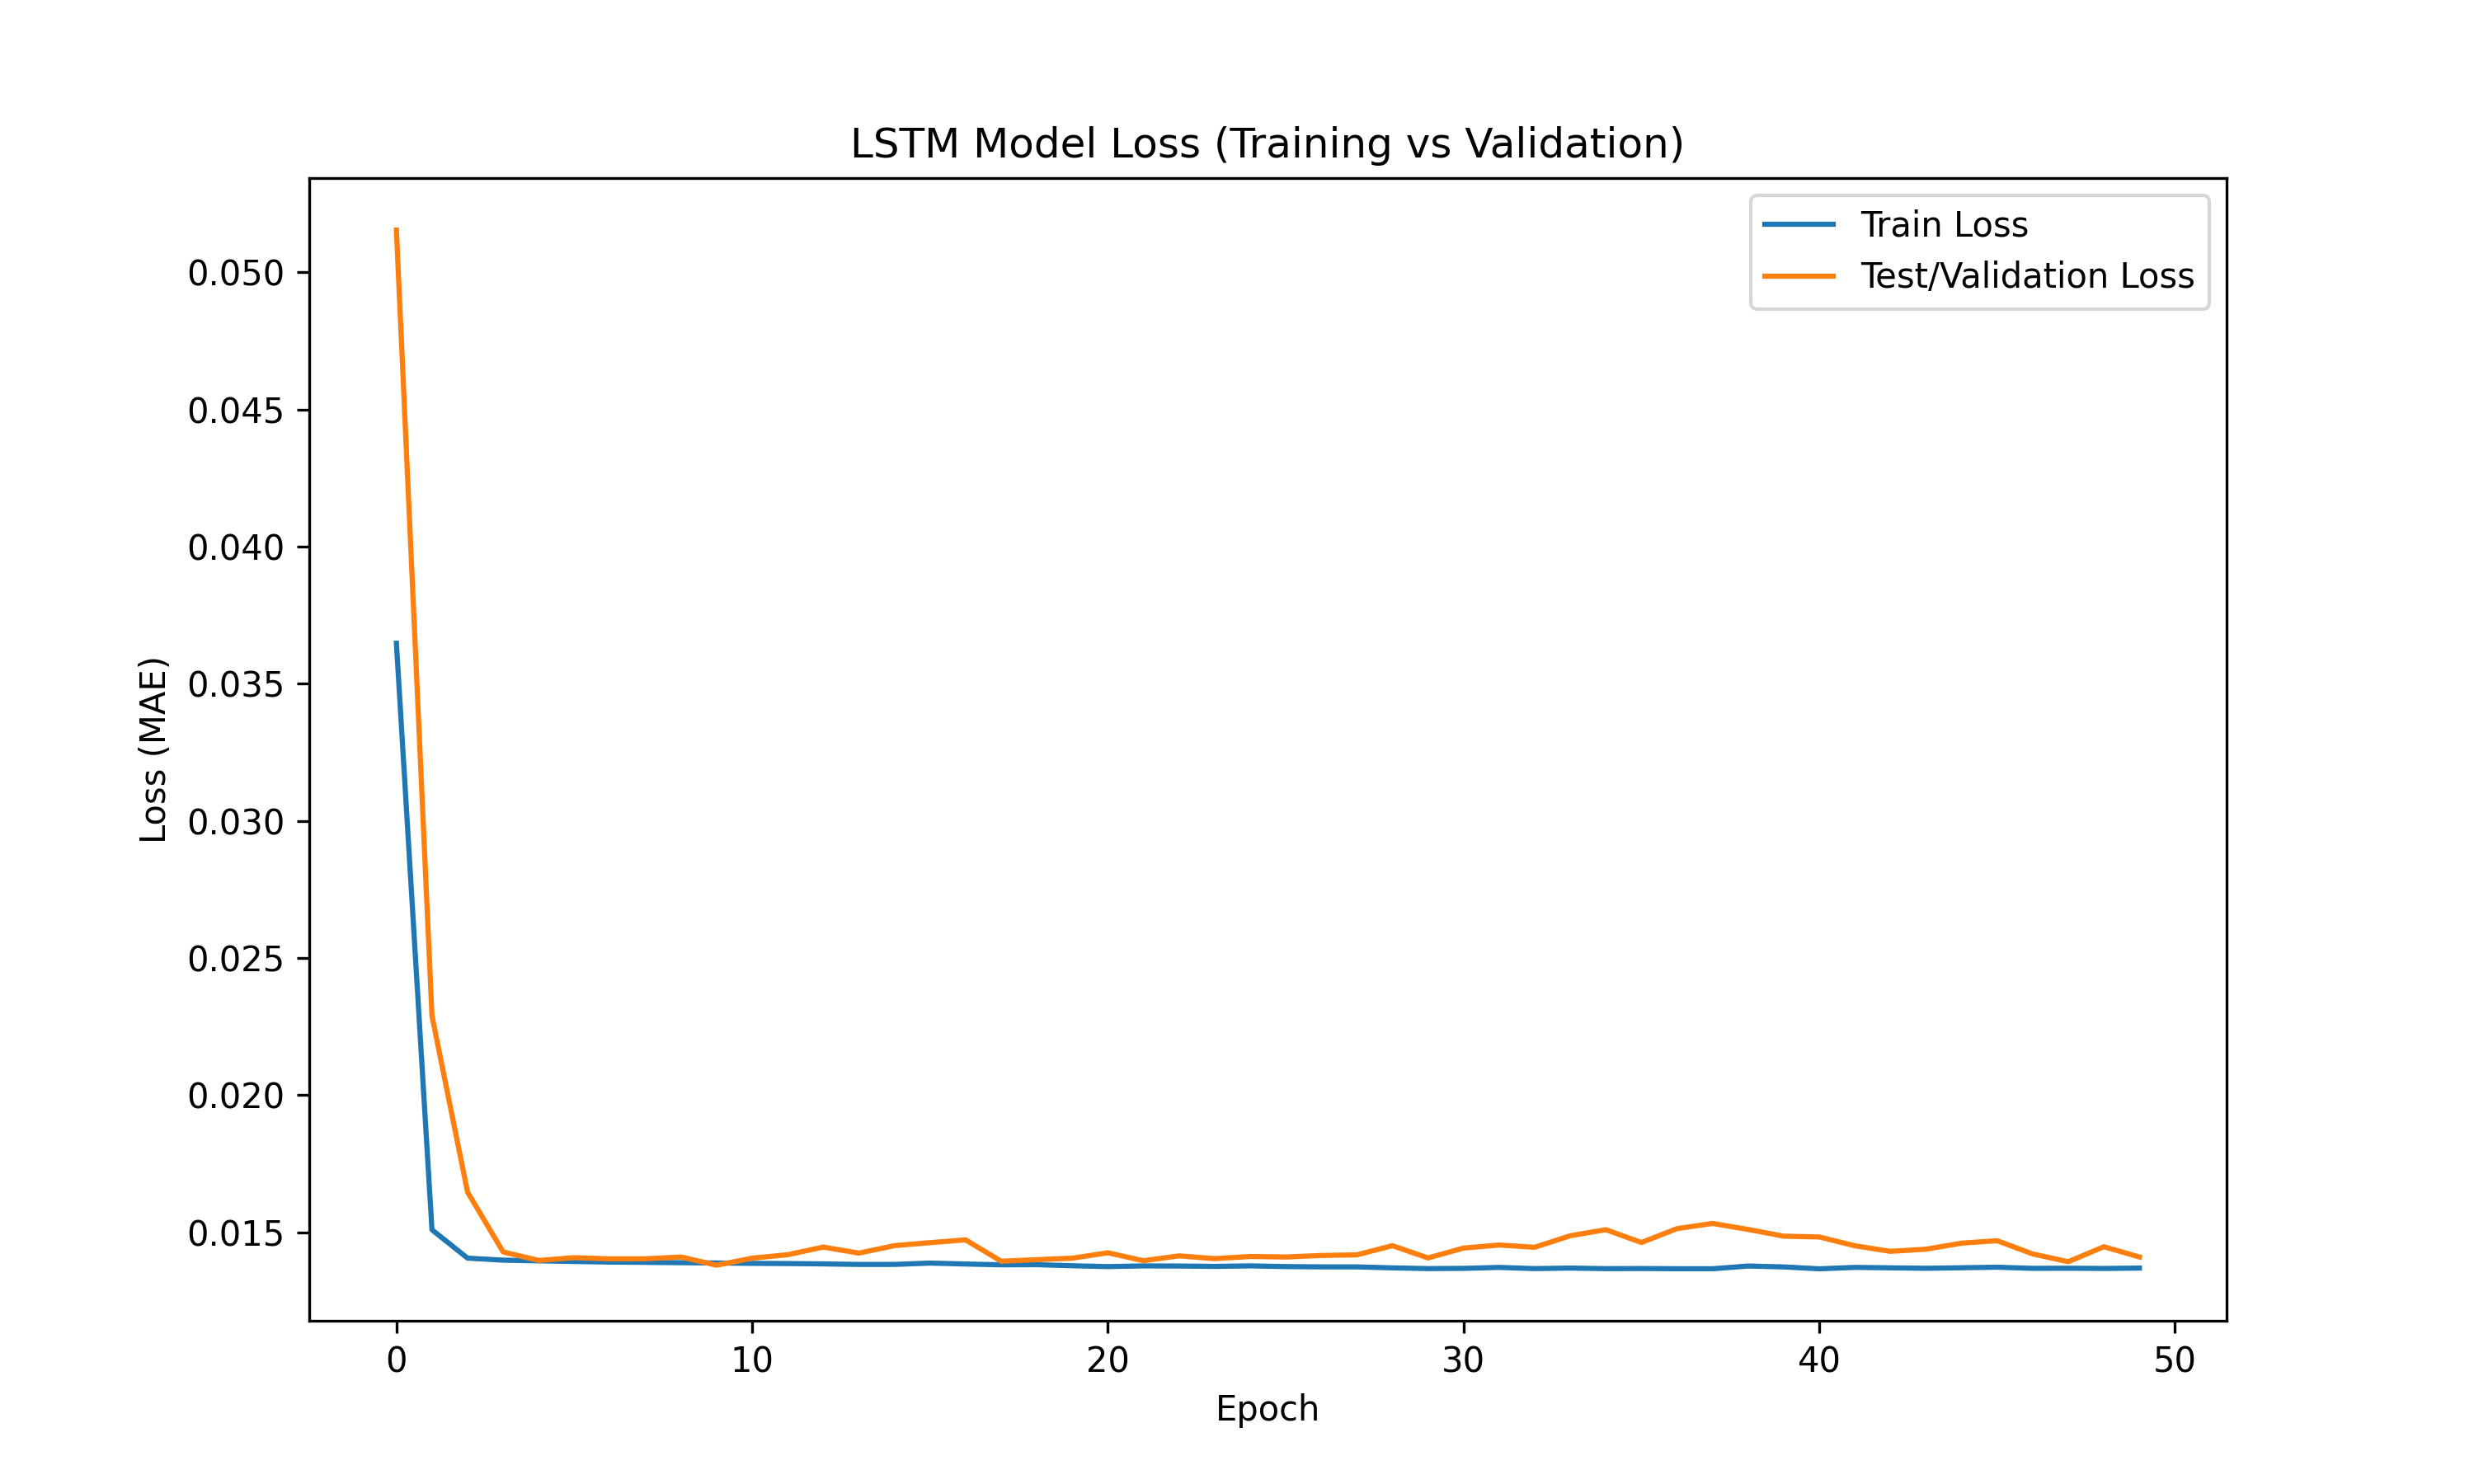
\includegraphics[width=0.85\textwidth]{lstm_loss.png}
    \caption{\textbf{LSTM Training vs. Validation Loss (MAE)}}
    \label{fig:loss}
\end{figure}

\subsection{Forecasting Evaluation}
After generating predictions on the test set (the 5th year), we inversely transformed the predicted and true arrays from the $[0, 1]$ scaled space back to the original PM2.5 concentration scale. The model achieved a final \textbf{RMSE of 25.663}. Considering that PM2.5 levels in the dataset can peak near 1000, an error margin of $\approx 25$ demonstrates extremely high precision.

\begin{figure}[H]
    \centering
    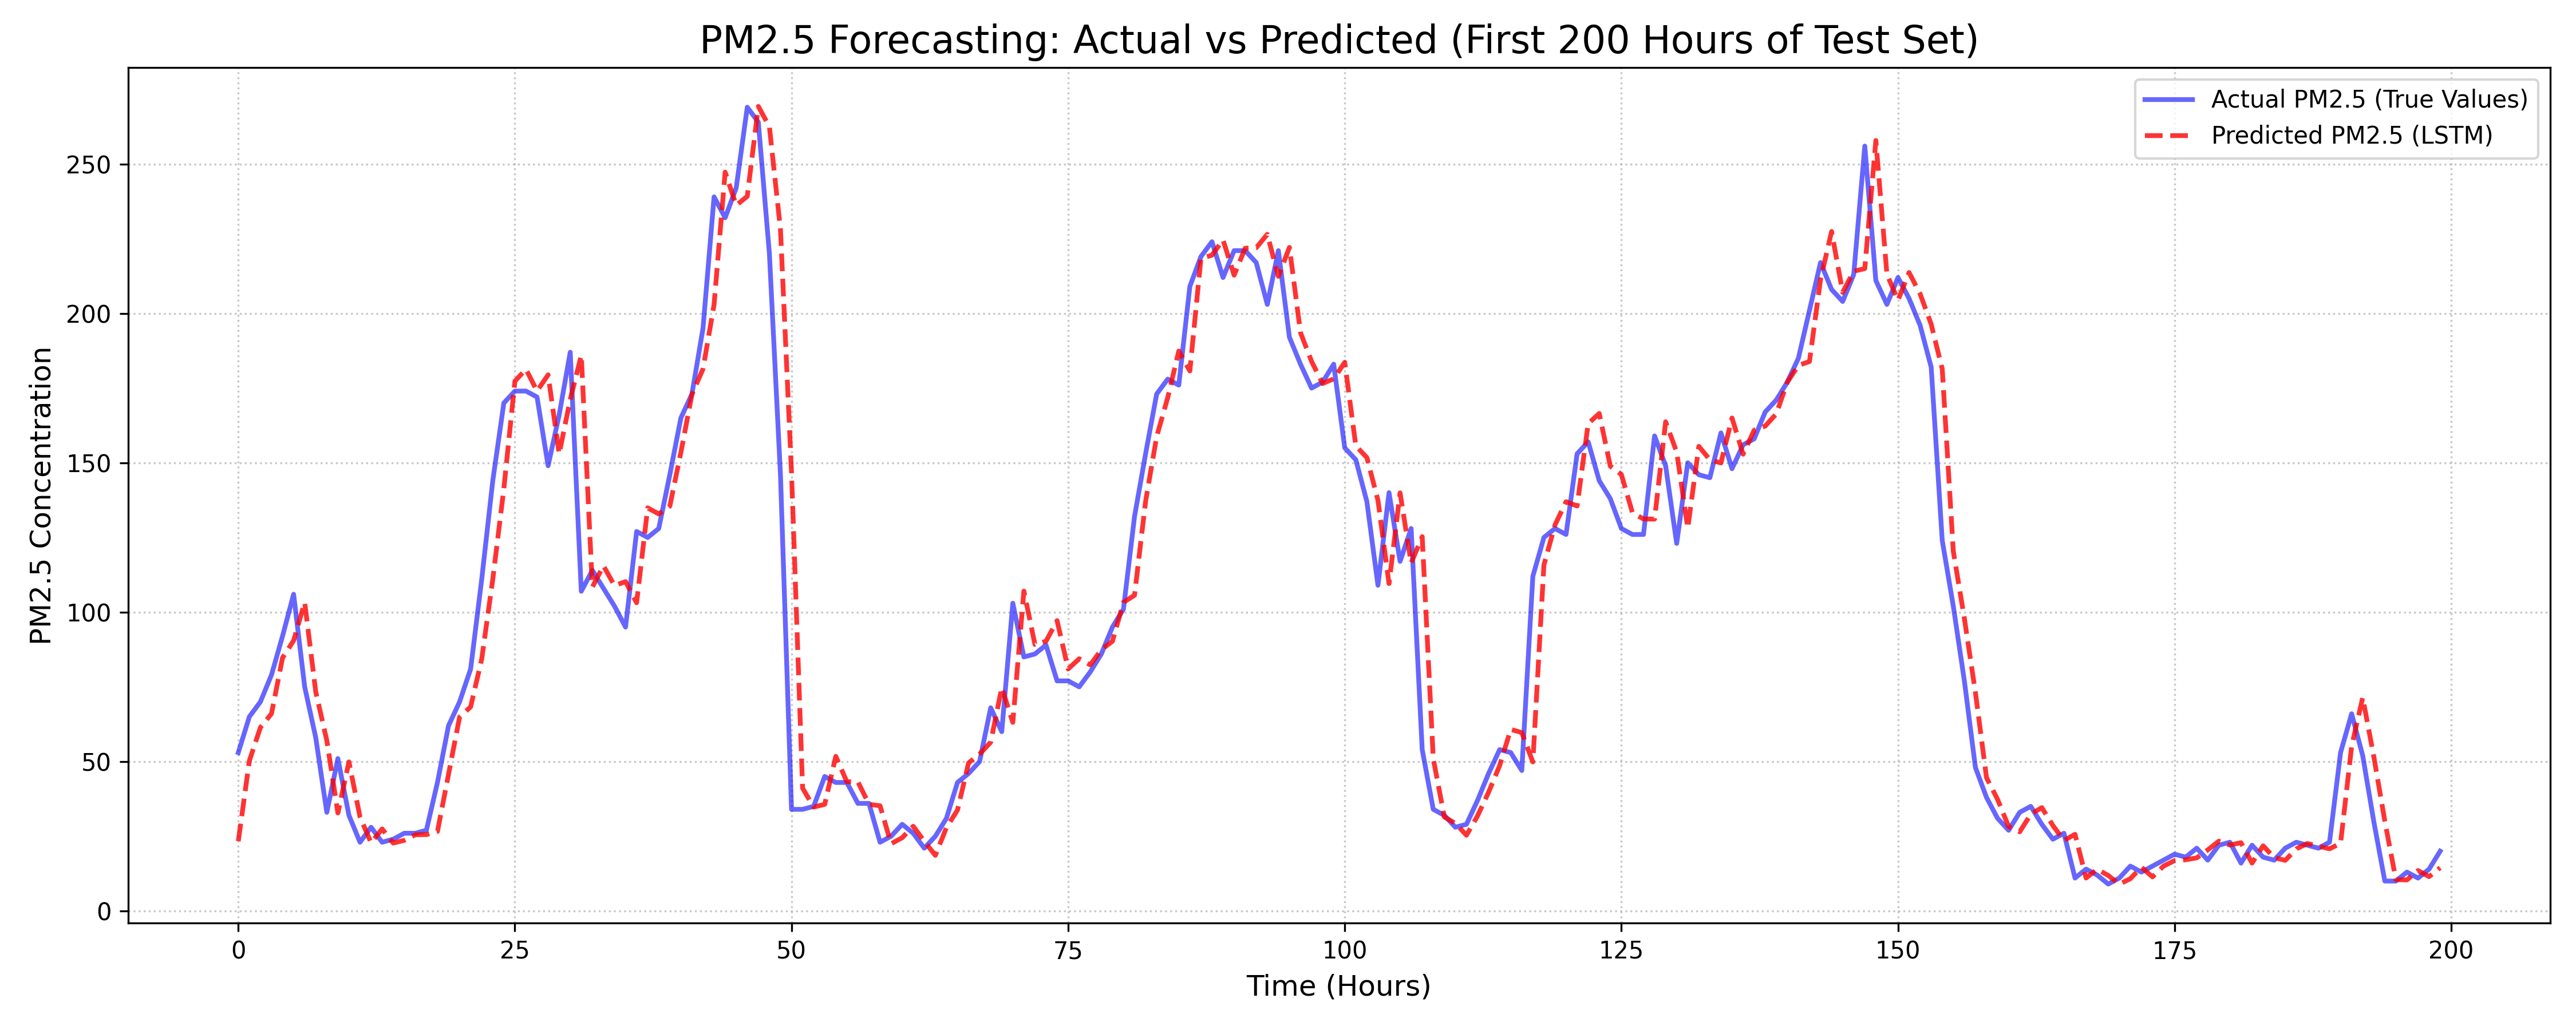
\includegraphics[width=\textwidth]{prediction_comparison.png}
    \caption{\textbf{Actual vs. Predicted PM2.5 Concentration (First 200 Hours of Test Set)}}
    \label{fig:prediction}
\end{figure}

As visualized in Figure \ref{fig:prediction}, the predicted trajectory (red dashed line) almost perfectly aligns with the ground truth (blue solid line). The LSTM successfully anticipated sharp volatility and inflection points, proving that it synthesized the underlying physics of wind dynamics and dew points to foresee pollution accumulation and dispersion.

\section{Conclusions}
This study validates the superiority of LSTM networks in handling multivariate time series data. By properly encoding, scaling, and framing environmental sensor arrays into sequence tensors, the neural network effectively captured the hidden correlations between weather conditions and pollution. The low RMSE and high curve-fitting accuracy underscore the potential of deep learning architectures in creating reliable, early-warning environmental forecasting systems.

\newpage
\phantomsection
\addcontentsline{toc}{section}{References}
\begin{thebibliography}{99}
    \bibitem{hochreiter1997} Hochreiter, S., \& Schmidhuber, J. (1997). \textit{Long short-term memory}. Neural computation, 9(8), 1735-1780.
    \bibitem{kaggleDataset} Roy, R. \textit{Air Pollution Forecasting - LSTM Multivariate}. Kaggle Dataset. \url{https://www.kaggle.com/datasets/rupakroy/lstm-datasets-multivariate-univariate/data}
\end{thebibliography}

\end{document}